\section{Mesh}
Meshes are 3D shapes which consists of vertices, indices and polygons. Not only the characters and furnitures are such meshes, even all rooms are handled as such meshes. PixelLight has it's own, binary chunk based mesh format. Meshes consist of different geometries and therefore it's possible to have a mesh with different materials per geometry. You have full access to the mesh to get on each information such as current vertex position, replacing a material after explosion through a damaged one and so on. Meshes can be loaded using a mesh loader class, there's a native loader for the PixelLight mesh format. For other mesh formats, one can use the plugin \emph{PLAssimp}. This plugin is using \ac{ASSIMP} in order to provide loader implementations for 3ds, obj, Blender, Collada and so on. There are also mesh creator classes which can create new meshes like a sphere automatically.




\subsection{Mesh Handler and Loose Meshes}
You should use mesh handlers in order to use mesh and to access their data over this provided interface. To load up a mesh do this:

\begin{lstlisting}[caption=Loading a mesh]
PLMesh::Mesh *pMesh = pMyMeshManager->LoadMesh("MyMesh.mesh");
PLMesh::MeshHandler cMeshHandler;
cMeshHandler.SetMesh(pMesh);
\end{lstlisting}

The mesh manager then will load up the mesh if it's not already loaded. There's also a function that unloads the mesh but this normally isn't required because that's done automatically when loading a new mesh or when the mesh handler is destroyed.




\subsection{Skeleton}
Each mesh can have a skeleton assigned to it. You can access it using the mesh handler function \emph{GetSkeletonHandler()}. A skeleton is a set of connected joints vertices connected to. By manipulating a joint, all children and vertices of the joint will be manipulated, too.

\begin{figure}
	\centering
	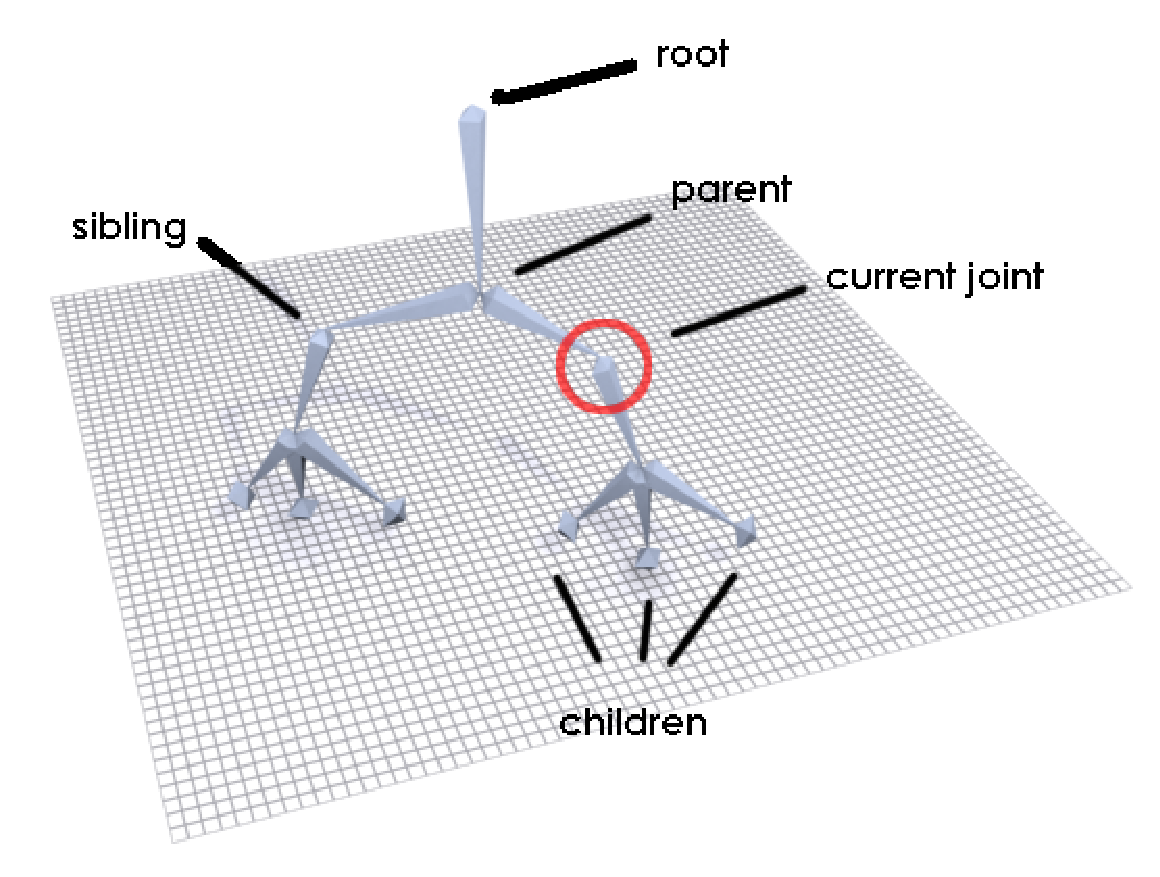
\includegraphics[scale=0.5]{pics/Skeleton.eps}
	\caption{Skeleton}
	\label{fig:Skeleton}
\end{figure}




\subsection{Animations}
Meshes can have morph target or skeletal\footnote{Also called, vertex/palette skinning} animations which can be mixed together. There's no limitation about the number of mixed animations, but try to avoid playing thousands of animations at the same time - the performance would be terrible. The animation playback itself is handled over a comfortable uniform animation interface.

You can use the \emph{GetAnimationsList()} function of the mesh handler to request a list of all available animations - note that there's no difference between morph target and skeleton animations. Because you as programmer should not be forced to create animations by self, that's the task of the graphic designer - this will safe you a lot of time! But the creation of own animations during runtime by hand is still possible. The animation resources are accessed through their names set by the designer like \emph{stand}, \emph{walk} an so on, they can be accessed trough their ID, too, but that's not recommended! To be able to playback such animation resources your mesh handler needs an animation manager which is a kind of mixer, it mixes the currently played animations to get a final result. The software animation manager is the default setting - this manager has no real limited features but it is using the \ac{CPU}. A hardware animation manager\footnote{Not yet implemented} would be another known alternative, which may have a better performance, but such managers normally have different limitations like a weights per vertex limit, a joint limit, active morph targets limit etc. The following example creates an animation manager instance if there's no one and start's the playback of all available animations:

\begin{lstlisting}[caption=Animation playback]
// Get/create the animation manager of our mesh handler
PLMesh::MeshAnimationManager *pAniManager = pMeshHandler->GetMeshAnimationManager();
if (!pAniManager)
	pAniManager = pMeshHandler->CreateMeshAnimationManager();
if (pAniManager) {
	// Get a list of all available animations
	PLCore::Array<PLCore::String> lstAnimations;
	pMeshHandler->GetAnimationsList(lstAnimations);
	for (PLCore::uint32 i=0; i<lstAnimations.GetNumOfElements(); i++) {
		PLMesh::AnimationInfo *pAniInfo = pMeshHandler->GetAnimationInfo(*lstAnimations[i]);
		PLMesh::Animation *pAni = pAniManager->Create(*lstAnimations[i]);
		if (pAniInfo && pAni)
			pAni->Start(pAniInfo);
	}
}
\end{lstlisting}

\begin{figure}
  \centering
  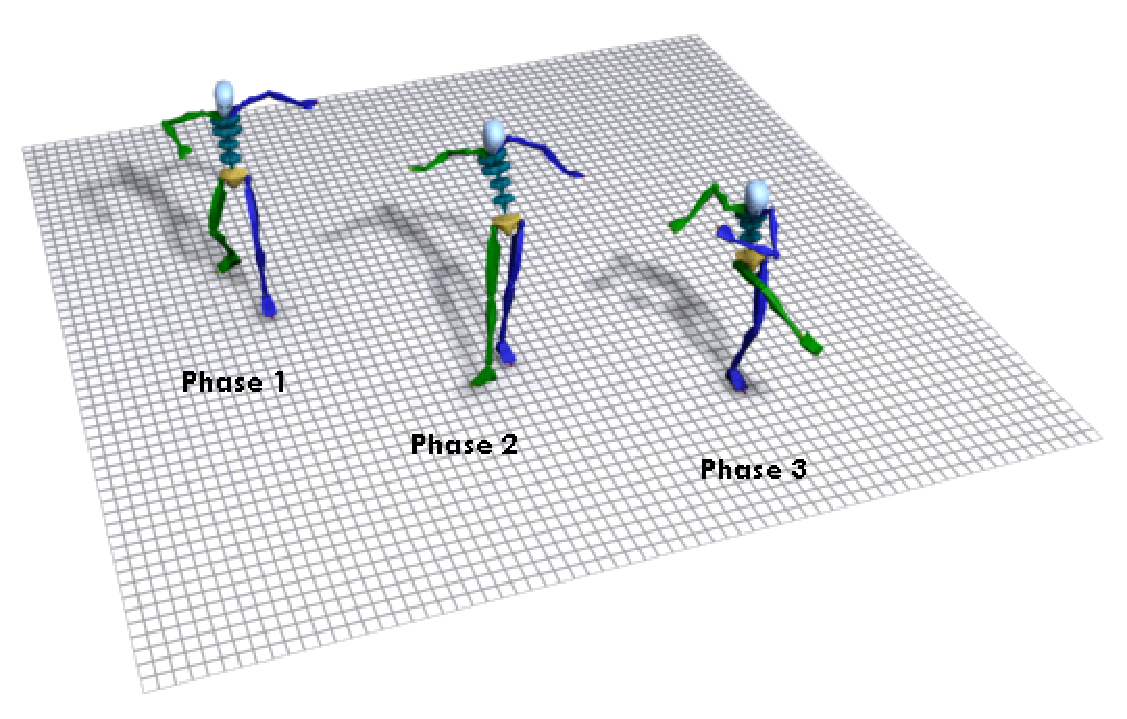
\includegraphics[scale=0.5]{pics/Joints.eps}
  \caption{Skeleton animation}
  \label{fig:Skeleton animation}
\end{figure}
